
\documentclass{template/socthesis}

%\usepackage[left=35mm, right=30mm]{geometry}
\usepackage{subcaption}

\graphicspath{ {./images/} }

\addbibresource{sources.bib}

% Title Page
\titlesk{BrailleFeeder - pomôcka pre zrakovo postihnutých}
\school{Stredná odborná škola}
\address{Športová 675, 916 01 Stará Turá}
\author{Juraj Kulich}
\mentor{}
\field{18}


\begin{document}
	
\maketitle
\makecopyrightstatement{V Novom Meste nad Váhom}
\makethanks{Ďakujem svojmu spolužiakovi Romanovi Mariančíkovi za obetavú pomoc, podmetné  pripomienky a nekonečnú trpezlivosť, ktorú mi počas práce poskytoval.}

\tableofcontents

\chapter*{Úvod}
\addcontentsline{toc}{chapter}{Úvod}
V roku 2015 malo približne 441 milónov ľudí zrakové postihnutie. Z toho bolo 36 milónov ľudí slepých \cite{bourne2017magnitude}. Takíto ľudia môžu použiť namiesto klasického textu Braillovo písmo, avšak drvivá väčšina pomenovaní a názvov je v klasickom písme. Takisto nikde nenájdeme noviny v Braillovom písme.

TODO

Aplikácia beží na systéme Android. Na tomto systéme beží celosvetovo už cez 2 miliardy aktívnych zariadení \cite{ng_2017}. Náš systém beží na minipočítači, na ktorom je platforma Android Things, ktorá je taktiež založená na Androide. Z toho dôvodu môžeme našu aplikáciu implementovať aj na mobilné zariadenia, na ktoré však nemôžeme pripojiť periférie a tak je funkčnosť obmedzená.
\newpage

\chapter*{Cieľ práce}
\addcontentsline{toc}{chapter}{Cieľ práce}
\newpage

\chapter*{Metodika práce}
\addcontentsline{toc}{chapter}{Metodika práce}
\newpage

\chapter{Braillovo písmo}
Braillovo písmo je druh písma určeného pre nevidiacich a slabozrakých. Funguje na princípe vyvýšených bodov, ktoré sa dajú čítať hmatom. Zhotovil ho slepý Louis Braille pôvodne z vojenského písma. 

Jedno písmeno Braillovho písma tvorí obdĺžnik bodov s dvoma stĺpcami a troma riadkami, ktorý sa nazýva braillovská bunka. Písmeno Braillovho písma je vo veľkosti rozmeru ukazováka, keďže na brušku ukazováka je najcitlivejší prah hmatu.
Na bunke je možné vytvoriť 64 znakov vrátane prázdnej bunky, ktorá tvorí medzeru. 
Základnú sadu tvoria písmená malej abecedy a interpunkčné znamienka. Čísla a veľké písmená sa tvoria pomocou prefixov.  Napríklad písmeno „c”,  „C” a číslo 3 sa zapíšu tým istým znakom, na rozoznanie sa však používa prefixový znak (Obr. 1.1).

\begin{center}
	\begin{figure}[htp]
		\centering
		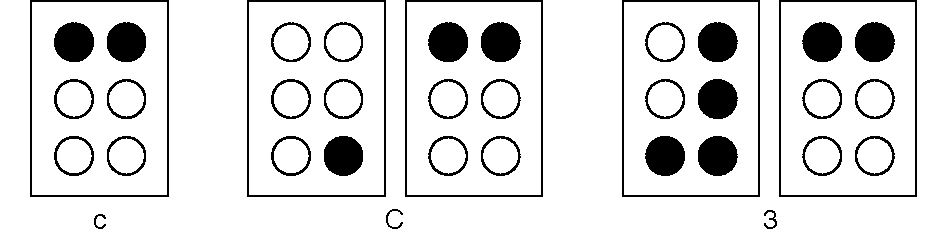
\includegraphics[scale=0.8]{braille}
		\caption{Príklady písmen s ukážkou prefixov}
	\end{figure}
\end{center}

Naše písmeno je však z dôvodu elektronického a veľmi lacného prevedenia(približne 19) väčšie ako je národná norma. Napriek tomu je však použiteľné. Na porovnanie, výrobná cena štandardizovaného článku je okolo 30 a je nemožné sa k takým kusom dostať.
\newpage
\chapter{Android Things OS}
Android Things je zjednodušená verzia operačného systému Android prispôsobená pre IoT zariadenia. Je navrhnutý tak aby fungoval v inteligentných zariadeniach, napríklad termostatoch alebo kamerách.

\section{IoT - Internet of Things}
Internet of Things, v preklade internet vecí, v informatike označuje sieť fyzických zariadení, vozidiel, domácich spotrebičov a ďalších zariadení, ktoré môžu byť vybavené elektronikou, softvérom, senzormi a sieťovou konektivitou, ktorá týmto zariadeniam umožňuje vzájomné prepojenie a výmenu dát. \cite{karimi2013internet}
\section{Android OS}
Android je open source operačný systém pre mobilné zariadenia vyvíjaný spoločnosťou Google. Je postavený na jadre Linuxu. V tejto kapitole si ukážeme vlastnosti  a princípy tohto systému a spôsoby tvorby aplikácii pre tento systém.

\subsection{Základné princípy}
\subsubsection{Architektúra systému Android}

Architektúra systému Android je rozdelená do niekoľkých vrstiev (Obr. 2.1) pričom každá vrstva využíva služby vrstvy pod ňou. 
\begin{center}
	\begin{figure}[htp]
		\centering
		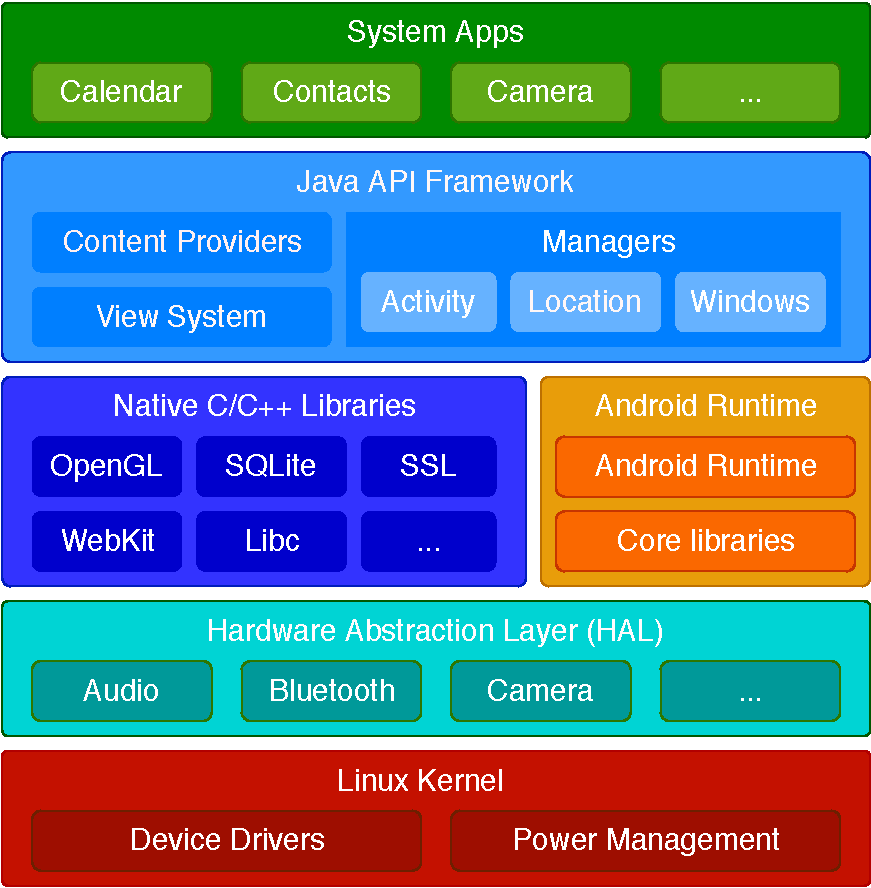
\includegraphics[scale=0.80]{android_architecture}
		\caption{Architektúra systému Android}
	\end{figure}
\end{center}

Vrstvy začiatkom od spodnej sú \cite{gandhewar2010google}\cite{androiddevelopers}:
\begin{itemize}
	\item Linux Kernel -- Jadro systému, ktoré poskytuje systémové služby ako sú bezpečnosť, správa pamäte, procesov, sietí a driverov. Slúži taktiež ako abstraktná vrstva medzi hardvérom a softvérom.  
	\item Hardware Abstraction Layer (HAL) -- Hardvérová abstraktná vrstva, ktorá poskytuje štandardné rozhrania vyššej vrstve. Skladá sa z rôznych knižníc, z ktorej kazdá implementuje rozhranie pre špecifický komponent, napríklad kameru alebo Bluetooth.
	\item Libraries -- Obsahuje knižnice písané v jazykoch C a C++. Sú volané cez Java rozhranie. Obsahujú knižnice pre zobrazovanie okien, jadrá pre 2D alebo 3D grafiku, kodeky ako MP3 alebo MPEG-4, SQL databázu alebo WebKit - renderovacie jadro pre prehliadače. 
	\item Android Runtime -- Obsahuje základné knižnice, ktoré poskytujú väčšinu funkcií dostupných v knižniciach jazyka Java. Ďalej obsahuje aplikačný virtuálny stroj Dalvik. 
	
	Virtuálny stroj \textit{Dalvik} -- Vytvára runtime prostredie pre Java aplikácie. Java aplikácie sa najprv prekladajú do bajtkódu pre virtuálny stroj Java, ten sa prekladá do bajtkódu Dalvik a ukladá do súborov .dex - Dalvik Executable a .oed - Optimized Dalvik Executable. Tieto súbory sú menšie a efektívnejšie na Android zariadeniach, ktoré majú slabší procesor a pamäť. Dalvik vytvára pre každú aplikáciu samostatnú inštanciu virtuálneho stroja.  
	 
	\item Java API Framework -- Obsahuje sadu funkcií v jazyku Java potrebných pre tvorbu mobilných aplikácií.
		\begin{itemize} 
		\item View System -- Poskytuje rozhranie pre stavbu užívateľského prostredia
		\item Resource Manager -- Poskytuje prístup k externým zdrojom ako sú reťazce, grafické prvky a súbory s~rozložením prostredia. 
		\item Notification Manager -- Poskytuje prístup k zobrazovaniu notifikáciam v stavovom riadku.
		\item Activity Manager -- Riadi životný cyklus aplikácie.
		\item Content Provider -- Umožňuje zdieľať dáta ostatným aplikáciam.
		\end{itemize}
	\item System Applications -- Je to najvyššia vrstva, ktorá poskytuje množstvo základných aplikácií ako sú email, SMS program, kalendár, aplikácie tretích strán a podobne.
\end{itemize}

\section{Použité technológie}
Na vývoj hlavného programu bol použitý jazyk Java z dôvodu predchádzajúcich skúseností s týmto jazykom a veľmi rozšírenou komunitou.

Na vývoj softvéru sme použili oficiálne vývojové prostredie od Googlu - Android Studio. Toto prostredie je postavené na vývojovom prostredí IntelliJ IDEA, podporuje dopĺňanie príkazov, refaktoring alebo analýzu kódu. Toto prostredie obsahuje aj emulátor, ktorý slúži ako virtuálne Android zariadenie.

\subsection{Použité knižnice}
\subsubsection{Butterknife}
Knižnica Butterknife generuje k prvkom z rozhrania(napr. tlačidlo) štandardizovaný kód, čím nám skracuje dĺžku kódu a robí ho prehľadnejším.
\subsubsection{OkHttp}
Knižnica OkHttp slúži na posielanie a prijímanie HTTP a HTTP/2 požiadavok a prijímanie/spracovávanie odpovedí zo servera.
\subsubsection{Retrofit}
Retrofit je REST (Representational State Transfer) klient s typovou kontrolou. REST je rozhranie, ktoré definuje metódy pre prístup k dátam - vytvoriť, zmazať, upraviť, získať. Pomocou neho získavame dáta z internetu a ukladáme do našich Java tried.
\subsubsection{Room}
Poskytuje abstraktnú vrstvu nad SQL databázou, umožňuje lepší prístup k databáze použitím menšieho množstva kódu a overuje dotazy na databázu.
\subsubsection{Cloud Vision API}
Umožnuje zistiť obsah z fotografie. Detekuje skupiny objektov a vecí (napr. rastliny, zvieratá, …) a extrahuje tlačený text.
\subsubsection{Cloud Speech-To-Text API}
Konvertuje audio do textu. Slúži na hlasové ovládanie.
\subsubsection{Cloud Translation API}
Poskytuje rozhranie na preklad textu. V našom prípade z angličtiny do slovenčiny. Toto API zatiaľ nepodporuje Android a preto posielame požiadavku na server s textom, ktorý chceme preložiť.
\newpage

\chapter{Architektúra systému BrailleFeeder}

\section{Vývojová doska}
Mozog zariadenia tvorí HW platforma NXP i.MX7D. Táto platforma obsahuje množstvo zberníc a pinov na pripojenie rôznych zariadení. Tu využívame USB na pripojenie mikrofónu, RJ45/Wi-Fi na pripojenie k internetu, konektor na pripojenie fotoaparátu, 3.5mm jack na pripojenie audio zariadení a univerzálne piny GPIO na pripojenie ostatných potrebných periférií(tlačidlá, cievky, …).
Táto platforma má procesor ARM Cortex-A7 - 1GHz, 512MB pamäte RAM a 4GB internú pamäť. Fotoaparát sa pripája pomocou MIPI CSI rozhrania.

\section{Časti elektroniky}
\subsubsection{Elektronické Braillovo písmeno}
Základným prvkom tejto vlastne vyrobenej periférie je 6 elektronicky ovládaných solenoidov usporiadaných do obdĺžnika - tvoria jedno Braillovo písmeno. V platforme sa články prekonvertujú do kombinácii núl a jednotiek, ktoré sa odosielajú na vstupy tohto zariadenia pomocou GPIO pinov, a podľa toho vytvoria vysúvaním dané písmeno. 

Solenoid je súčiastka, ktorej časť sa za pomoci magnetu a cievky dokáže vysúvať a zasúvať. Keďže naša platforma dokáže na jednom GPIO pine poskytnúť maximálny prúd okolo 20mA, napájanie je riešené pomocou externej batérie. Tým pádom potrebujeme 6 optočlenov a tranzistorov na zopínanie cievok.

\subsubsection{Batérie}
Slúžia na napájanie dosky a modulu s cievkami(Braillovo písmeno). Používame tri nabíjateľné 3400mAh 3.7V batérie typu 18650. Na napájanie dosky používame napäťový booster z 3.7V na 5V.

\subsubsection{GPIO piny}
General-purpose input/output - sú digitálne piny, ktoré dokážu slúžiť aj ako vstupy aj výstupy podľa potreby. Používame ich ako výstupy pre posielanie impulzov do cievok a ako vstupy pri tlačidlách. 

\subsubsection{USB vstup}
Slúži na pripojenie USB mikrofónu

\subsubsection{3.5mm jack}
Slúži na pripojenie audio zariadení pre hlasový výstup

\section{Režimy použitia}
So systémom môžeme pracovať vo viacerých režimoch
\begin{enumerate}
\item Prehrávanie článkov na Braillovom písmene -- článok sa rozdelí na písmená a každé písmeno sa skovertuje na príslušný kód, podľa ktorého sa zobrazí výstupe.
\item Prehrávanie článkov cez reproduktor.
\item Vstup pre základné úkony pomocou tlačidiel. 
\begin{itemize}
\item prepínanie článkov
\item nastavenie hlasitosti
\item nastavenie rýchlosti prepínania Braillovho písma.
\end{itemize}
\item Vstup pre rozšírené úkony cez mikrofón (hlasové ovládanie) -- hlasové ovládanie je z dôvodu gramatickej nestálosti slovenského jazyka dostupné iba v anglickom jazyku.
\begin{itemize}
\item prepínanie článkov dopredu/dozadu
\item nastavenie hlasitosti na presnú hodnotu
\item určenie kategórie vyhľadávaných článkov 
\item vyhľadávanie článkov o konkrétnej téme
\item uloženie článkov do offline pamäte
\item načítanie uložených článkov
\item vytvorenie snímku
\item zmena jazyka prostredia do slovenského jazyka
\item pomocný príkaz pre nápovedu
\end{itemize}
\end{enumerate}

\printbibliography[title=Zoznam použitej literatúry]

\end{document}          
